\label{chp:Method}
% 4.2. Data Acquisition
\section{Preprocessing}
\label{sec:preprocessing}
Wi-Fi signature data must be pre-processed to be used as an input in the proposed system.
In this study, only the magnitude of the complex signal was utilized due to device firmware issues with the phase value of the 2.4Ghz Wi-Fi signal~\cite{wang2015understanding}.
Second, the data must be made to be the same size. All signals have different lengths, so equal length sampling was used to ensure that all data had the same length.
Third, outliers must be addressed. Wi-Fi signals are interrupted by other electromagnetic radiation of which burst noise~\cite{wang2015understanding} can have significant effects. Thus, only data within one standard deviation of the median were analyzed to minimize the effects of burst noise.
% 4.3. Proposed Methodology
\section{Proposed Methodology}
\label{sec:methodology}
%purpose
This thesis proposed an identity verification system based on the Wi-Fi signals produced by in-air handwritten signatures (``Wi-Fi signature''). 
%function
Triplet networks which utilized ConvNet as the feature extractor were used to learn the direction-invariant deep representations of in-air signatures~\cite{hoffer2015deep}. KAR space learning was used to mine triplet inputs to achieve faster loss convergence~\cite{toh2018learning,toh2018gradient}. 
% figure
\begin{figure*}[!ht]
    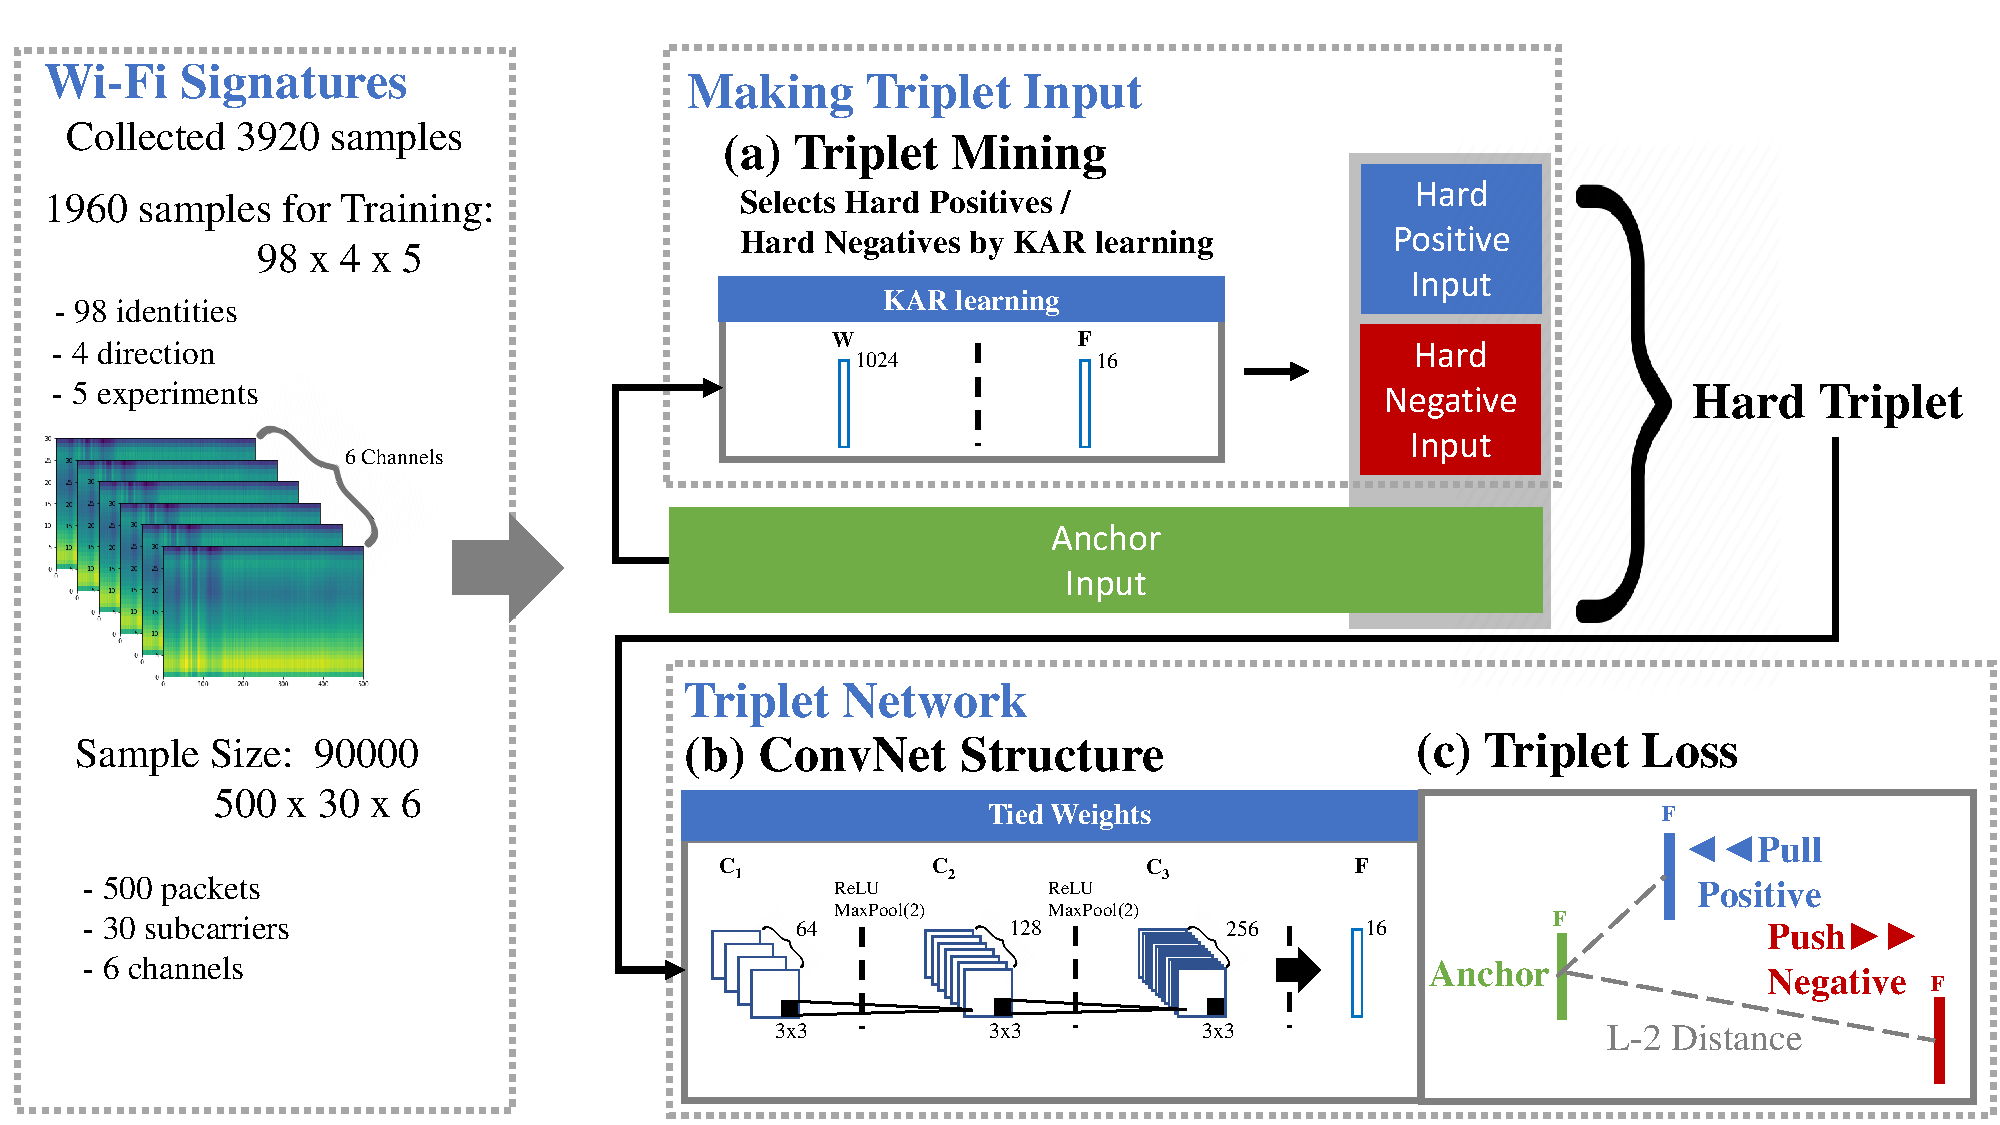
\includegraphics[width=\textwidth]
        {fig_system_overview_v1.pdf}
    \caption{An overview of the proposed methodology.} \label{fig1}
\end{figure*}
Figure~\ref{fig1} shows an overview of the proposed system. 
KAR space projection learning is used to mine hard samples from the training dataset to create triplets (Fig.~\ref{fig1}(a)). The anchor sample is randomly selected from the training dataset. The hard samples are those which are likely to be misclassified by the triplet network for a given anchor sample.
After the data is selected, the triplet network (Fig.~\ref{fig1}(b)) is trained based on the network output vector distance comparison (Fig.~\ref{fig1}(c)).
% following~
The following subsections discuss the triplet network architecture, triplet loss, and triplet mining using KAR space learning.

% 4.4.1. Triplet loss
\subsection{Triplet Loss}
% purpose
Triplet loss~\cite{hoffer2015deep} trains the ConvNet structure to learn the features that define data position in the feature space.
% Triplet input
Triplet inputs are composed of a combination of three samples, an anchor sample $x_0$, a positive sample $x_+$ and a negative sample $x_-$. The anchor sample, the reference for the triplet input, is selected from the training data set. The positive sample has the same identity as the anchor sample while the negative sample has a different identity.
% function
$dist\{f(x_0),f(x_+)\}$, the distance between the feature vectors of anchor $f(x_0)$ and positive sample $f(x_+)$ is larger than $dist\{f(x_0),f(x_-)\}$, the distance between feature vectors of the anchor and the negative sample plus a preset margin $\alpha$ to produce discriminative feature vectors. 
The distance measurement function is:
\begin{equation}
    dist\{f(x_0),f(x_-)\} - dist\{f(x_0),f(x_+)\} \geqq \alpha
    \label{triplet_condition}
\end{equation}
By using the $L2$ distance as the distance function, triplet loss is defined as:
\begin{equation}
    triplet\_loss = \sum_i^N max\left({ \left[ {\left\| {{f(x_0)} - {f(x_+)}} \right\|_2^2} - {\left\| {{f(x_0)} - {f(x_-)}} \right\|_2^2}  + \alpha \right]},0 \right),
    \label{triplet_loss}
\end{equation}
% need to make hard triplets
Note that if $dist\{f(x_0),f(x_-)\}$ is much larger than $dist\{f(x_0),f(x_+)\} + \alpha$, the output of the loss function is zero, significantly slowing deep network convergence. This condition is likely to occur if triplets are composed by randomly selecting training samples. Thus, triplet inputs must be selected that cause the loss function to produce a non-zero result.

% 4.4.2. Triplet mining
\subsection{Triplet Mining Based on KAR Space Learning}
% purpose
To train the triplet network faster, a sub-network for mining the hard positive and negative samples from the training dataset was trained.
% hard sample
The hard positive sample is likely to be misclassified as a negative sample by the triplet network (Fig.~\ref{fig2}).
The distance between the feature vectors of the anchor and hard positive samples is larger than other positive samples.
The hard negative sample is likely to be misclassified as a positive sample because the distance between the feature vectors of the anchor and the hard negative sample is smaller than the difference between the feature vectors of the anchor and other negative samples.
Hard triplet inputs are made by combining hard positive and hard negative samples with selected anchor samples. Using hard triplets as triplet network inputs more easily, satisfies~\ref{triplet_condition}. However, before training the triplet network, it is impossible to identify hard samples.
% figure
\begin{figure*}[!ht]
    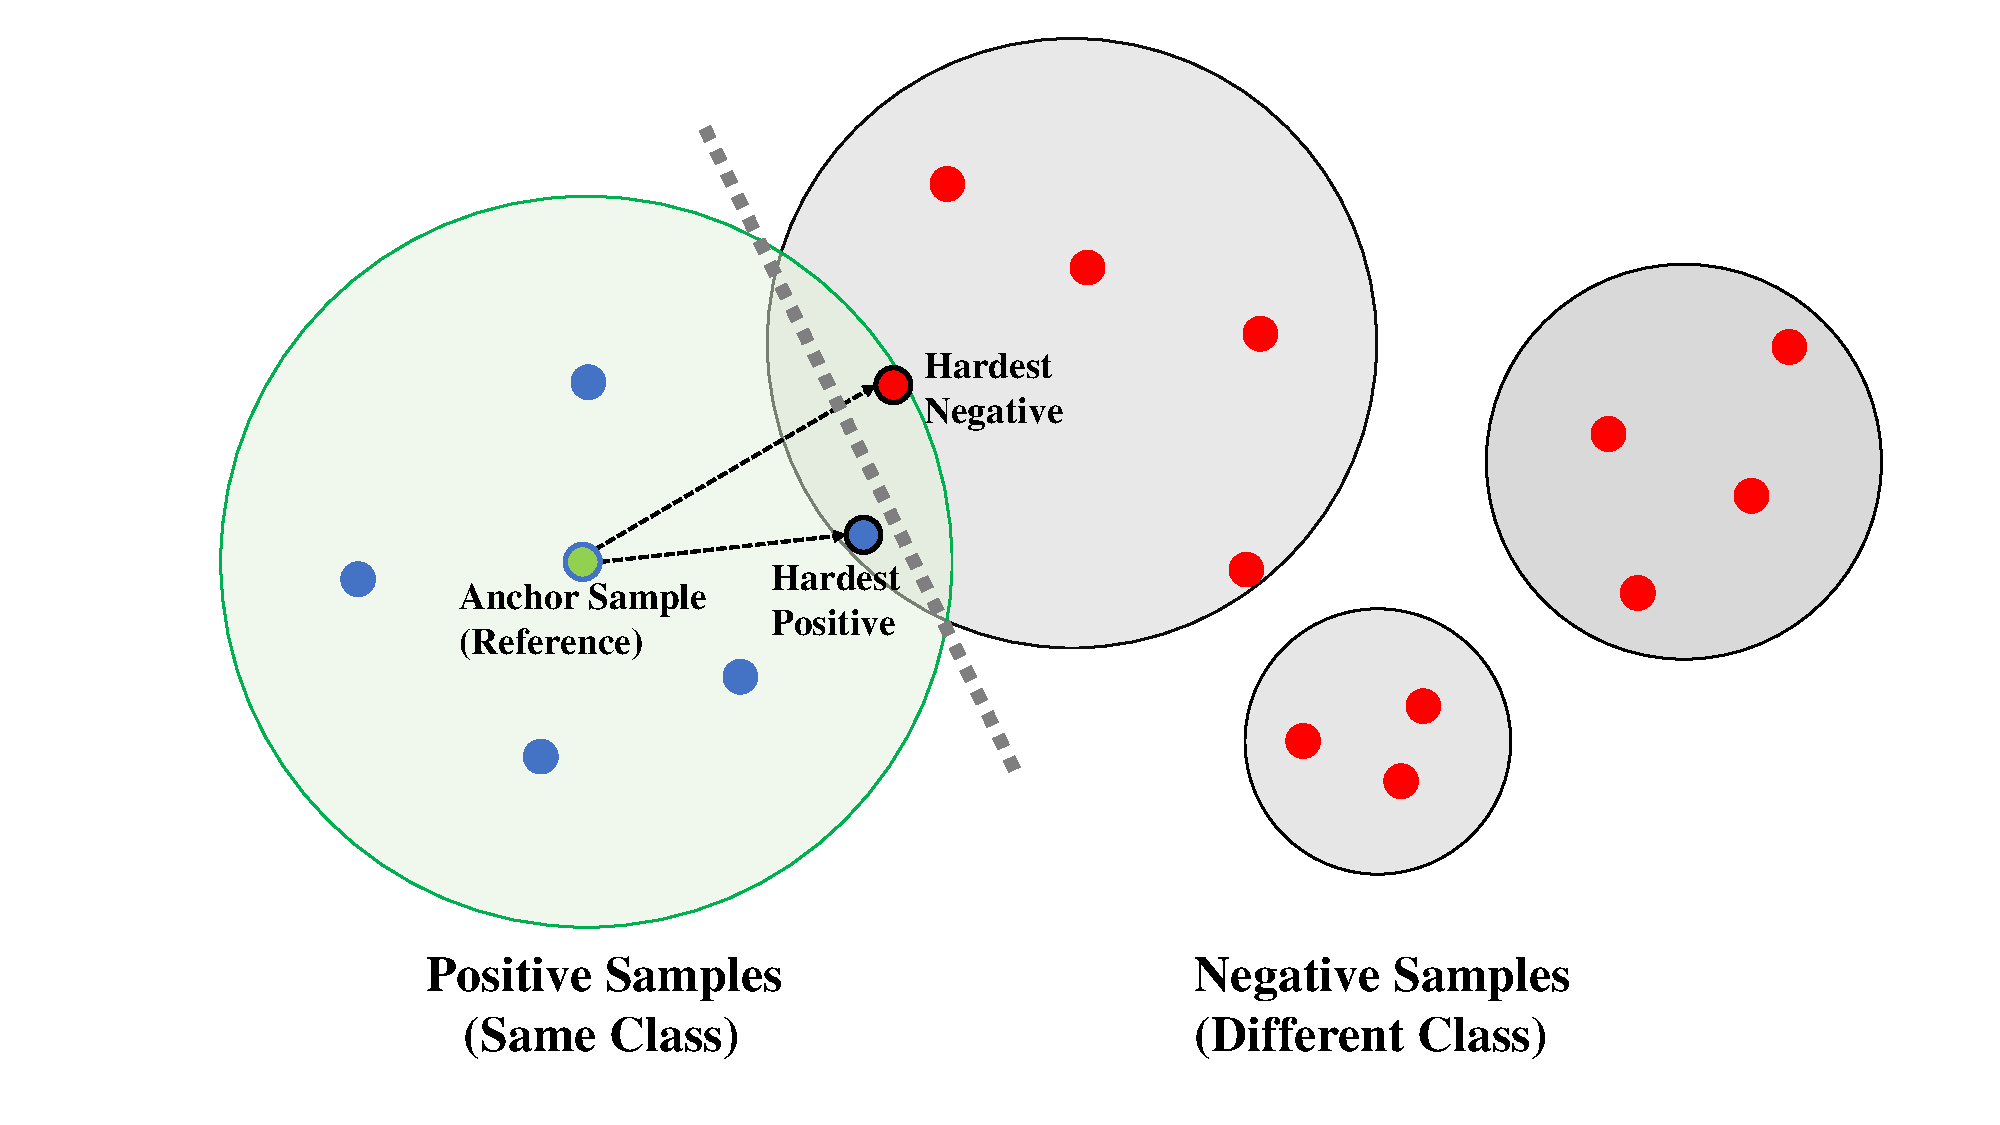
\includegraphics[width=\textwidth]
        {fig_hardsample_v2.pdf}
    \caption{Selection of hard samples.} \label{fig2}
\end{figure*}
% functions
In order to make hard triplets before tranining the triplet network, a smaller sub-network was trained before training the main triplet network.
This smaller sub-network was made of an MLP and was trained using KAR space learning. As KAR space learning has no backpropagation and no iterative learning process, it was trained all at once on the entire training dataset $X$. 
The sub-network output was defined as: 
\begin{equation}
    KAR\left(\mathbf{X}\right)=\sigma\left(\left[\mathbf{1},\sigma\left(\dots\left[\mathbf{1},\sigma\left(\left[\mathbf{1},\sigma\left(\mathbf{X}\cdot\mathbf{W}_{1}\right)\right]\mathbf{W}_{2}\right)\right]\dots\mathbf{W}_{(n-1)}\right)\right]\mathbf{W}_{n}\right).
\end{equation}
After training the sub-network, the hard samples were mined by measuring the $L2$ distance between every output vector of the sub-network and the output vector of anchor sample.
The sub-network output for a given anchor sample $x_0$ was $KAR(x_0)$. To mine hard-positive samples, one sample was selected from among the sub-network outputs for which the distance to the anchor feature vector $KAR(x_0)$ was larger than $t_+$. Hard-negative samples were chosen, from among the sub-network outputs for which the anchor feature vector was smaller than $t_-$.
The selected hard-positive and hard-negative samples satisfied the following properties, respectively:
\begin{equation}
    {\left\| {{KAR\left(\mathbf{x}_{0}\right)} - {KAR\left(\mathbf{x}_{+}\right)}} \right\|_2^2} \geq \mathrm{t}_{+}, 
    \label{thres_pos}
\end{equation}
\begin{equation}
    {\left\| {{KAR\left(\mathbf{x}_{0}\right)} - {KAR\left(\mathbf{x}_{-}\right)}} \right\|_2^2} \leq \mathrm{t}_{-},\label{thres_neg}
\end{equation}
If the hardest sample, outlier data is more likely to be selected than other data, resulting in an increased risk of overfitting~\cite{schroff2015facenet}.
To avoid this problem, the threshold for the hard-positive and the hard-negative samples were empirically chosen as the 25th and 75th percentiles of the distance between the anchor and sub-network outputs.

% 4.4.3. ConvNet Structures
\subsection{ConvNet Structures}
% Purpose
The three-dimensional format of the input signature signal is similar to that of image data, so deep ConvNet structures were used as the feature extractor. The ConvNets used in this thesis were made of three layers of ConvNets with triplet loss. Each layer of ConvNet shared their weights. 
% figure
\begin{figure*}[!ht]
    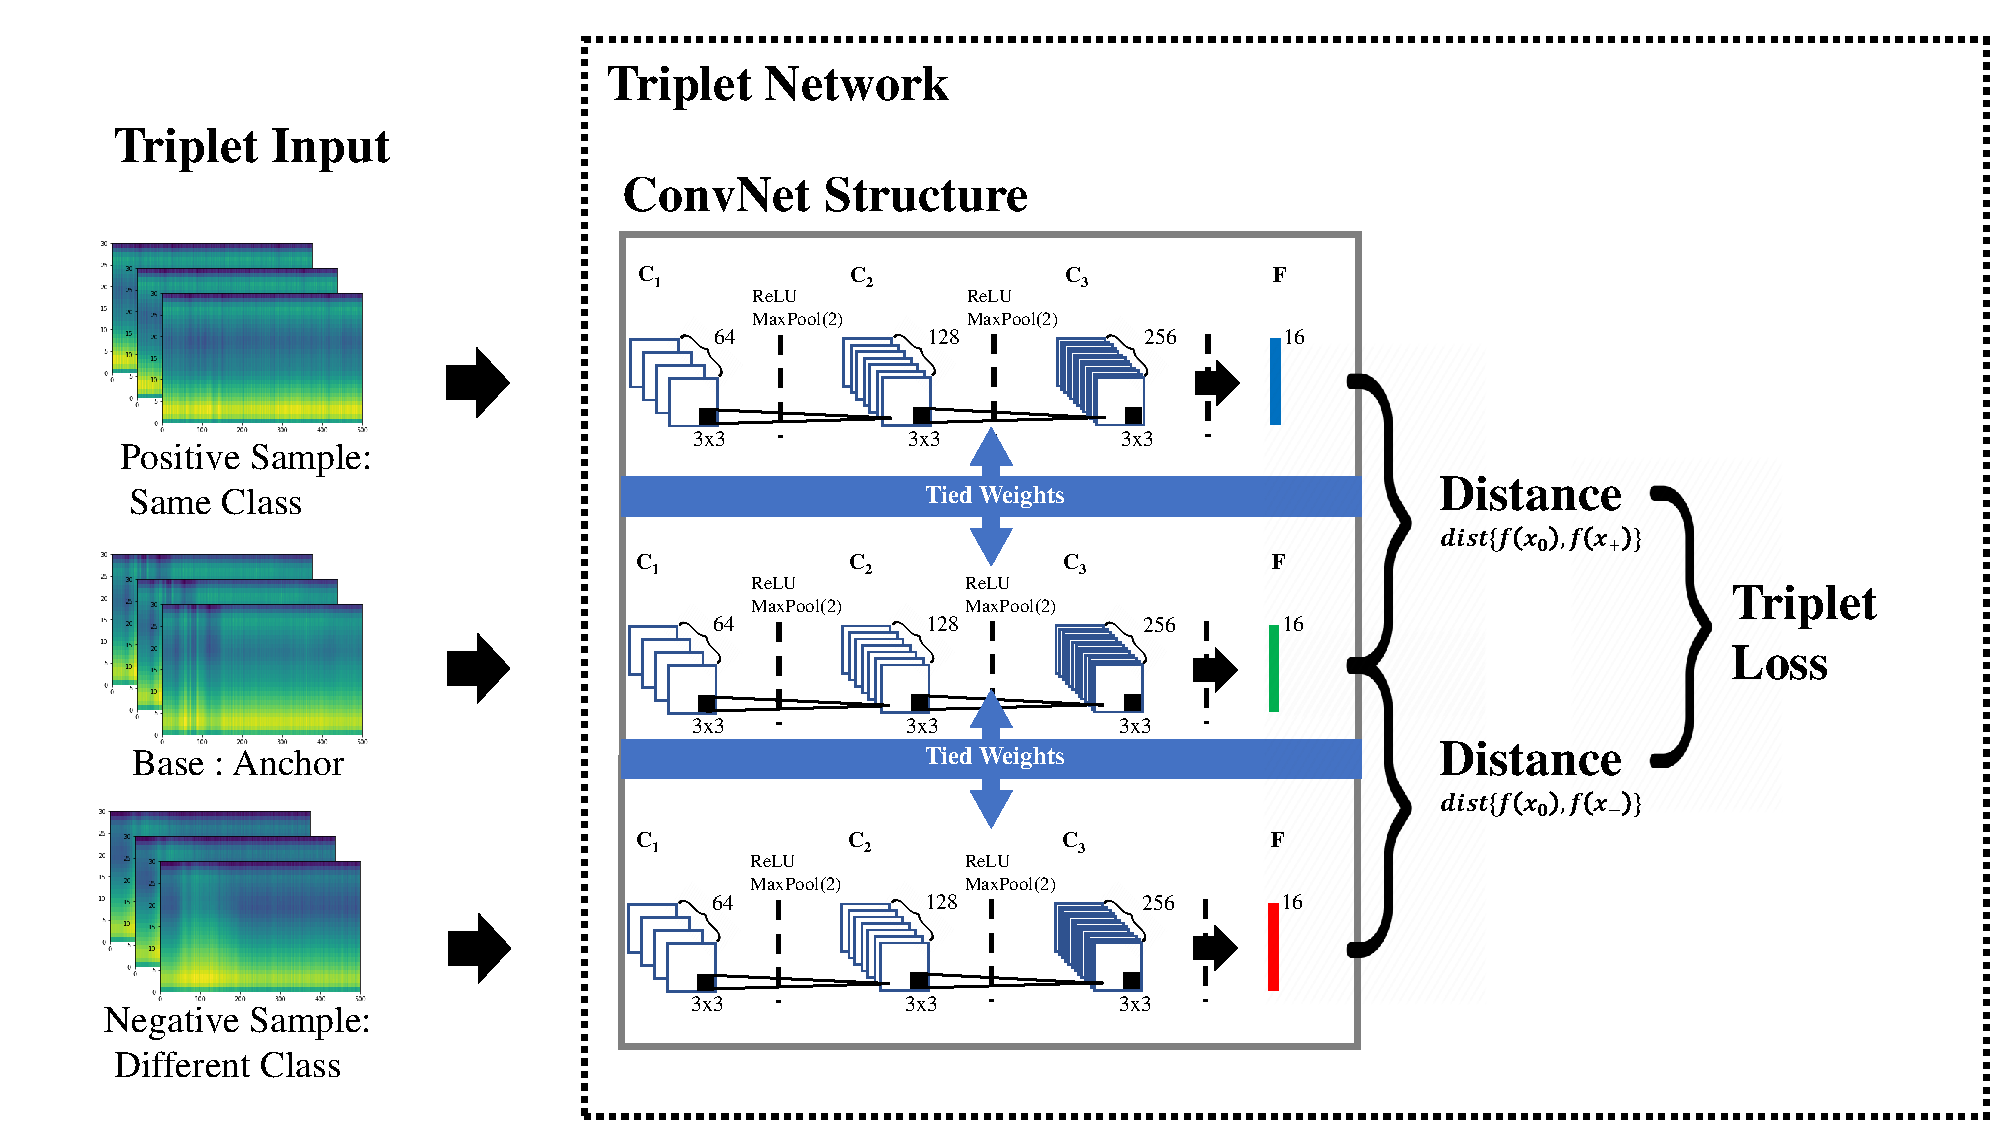
\includegraphics[width=\textwidth]
        {fig_convnet_v1.pdf}
    \caption{ConvNet structure.} \label{fig3}
\end{figure*}
% Structure
The ConvNets in this study consisted of three filters and a fully-connected output layer (Fig.~\ref{fig3}). The depth of the ConvNet filters was set at 64,128,256 with stride 1 and ReLU activation functions. The size of the fully-connected layer was 16. The fully-connected output layers were processed through sigmoid activation functions and were normalized according to the $L2$ distance.

